\documentclass[journal]{IEEEtran}
\usepackage[a5paper, margin=10mm, onecolumn]{geometry}
\usepackage{lmodern}

\setlength{\headheight}{1cm}
\setlength{\headsep}{0mm}

\usepackage{gvv-book}
\usepackage{gvv}
\usepackage{cite}
\usepackage{amsmath,amssymb,amsfonts,amsthm}
\usepackage{graphicx}
\graphicspath{{./figs/}}
\usepackage{xcolor}
\usepackage{txfonts}
\usepackage{enumitem}
\usepackage{mathtools}
\usepackage{hyperref}
\usepackage{tikz}
\usepackage{tkz-euclide}

\begin{document}

\bibliographystyle{IEEEtran}
\vspace{3cm}

\title{4.3.25}
\author{EE25BTECH11036 - M Chanakya Srinivas}
\maketitle

\renewcommand{\thetable}{\theenumi}
\setlength{\intextsep}{10pt}
\renewcommand\theequation{\arabic{equation}}



\section*{Question}
Find the ratio in which the line joining the points 
\[
\vec{A} = \myvec{-2 \\ 4 \\ 7}, \quad 
\vec{B} = \myvec{3 \\ -5 \\ 8}
\]
is divided by the YZ-plane.

\section*{Solution}

\subsection*{Step 1: Algebraic Derivation}
Let the direction vector be
\begin{align}
\vec{d} &= \vec{B} - \vec{A}.
\end{align}

The parametric equation of the line is
\begin{align}
\vec{R}(\lambda) &= \vec{A} + \lambda \vec{d}.
\end{align}

The equation of the YZ-plane is
\begin{align}
\vec{n}^\top \vec{x} &= 0, \quad 
\vec{n} = \myvec{1 \\ 0 \\ 0}.
\end{align}

Substituting $\vec{R}(\lambda)$,
\begin{align}
\vec{n}^\top \brak{\vec{A} + \lambda \vec{d}} &= 0.
\end{align}

Thus,
\begin{align}
\lambda &= -\frac{\vec{n}^\top \vec{A}}{\vec{n}^\top \vec{d}}.
\end{align}

If $P$ is the intersection point, then the section ratio is
\begin{align}
AP : PB &= \lambda : (1-\lambda).
\end{align}

---

\subsection*{Step 2: Numerical Substitution}
Now substitute the given coordinates:

\begin{align}
\vec{A} &= \myvec{-2 \\ 4 \\ 7}, \quad
\vec{B} = \myvec{3 \\ -5 \\ 8}, \\[1ex]
\vec{d} &= \vec{B} - \vec{A} = \myvec{5 \\ -9 \\ 1}.
\end{align}

\begin{align}
\lambda &= -\frac{\myvec{1 & 0 & 0}\vec{A}}
{\myvec{1 & 0 & 0}\vec{d}} 
= -\frac{\myvec{1 & 0 & 0}\myvec{-2 \\ 4 \\ 7}}
{\myvec{1 & 0 & 0}\myvec{5 \\ -9 \\ 1}} \\
&= \frac{2}{5}.
\end{align}

Hence,
\begin{align}
AP : PB &= \frac{2}{5} : \brak{1-\frac{2}{5}} = 2:3.
\end{align}

\[
\boxed{2:3}
\]

---

\subsection*{Step 3: Verification}
The intersection point is
\begin{align}
\vec{P} &= \vec{A} + \frac{2}{5}\vec{d} \\
&= \myvec{-2 \\ 4 \\ 7} + \frac{2}{5}\myvec{5 \\ -9 \\ 1} \\
&= \myvec{0 \\ \tfrac{2}{5} \\ \tfrac{37}{5}}.
\end{align}

Clearly, $x=0$, so $P$ lies on the YZ-plane.  
Thus, the ratio is verified as $2:3$.




\begin{figure}[h]
    \centering
    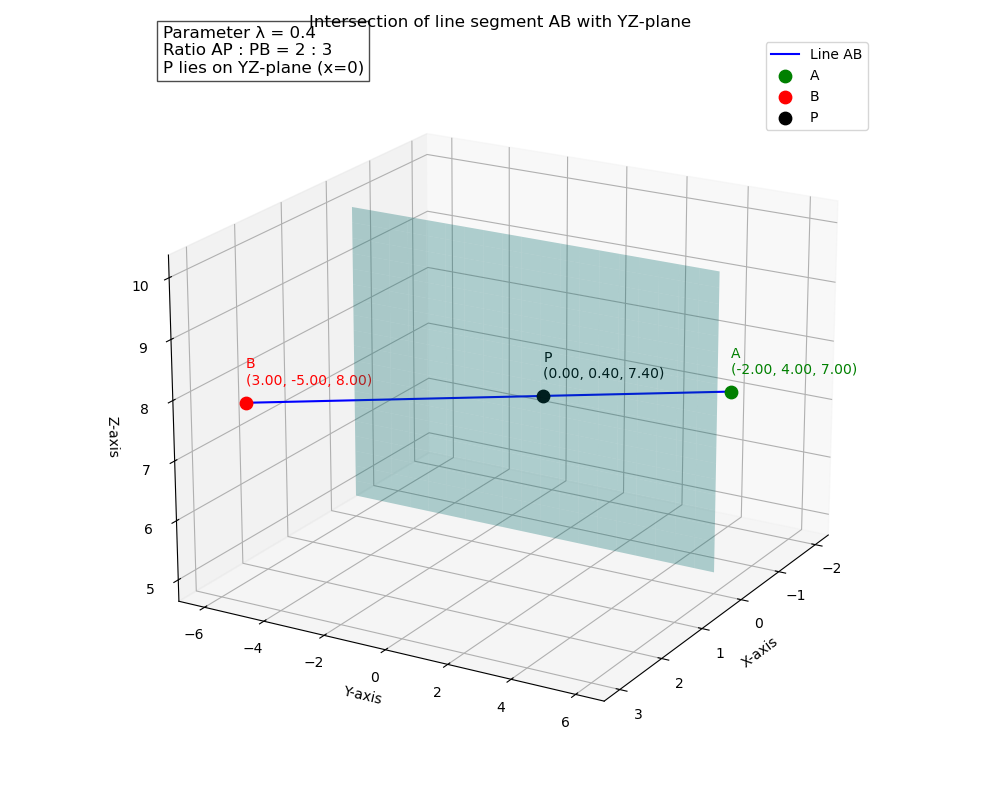
\includegraphics[width=0.9\columnwidth]{figs/fig_61.png}
    \caption{Line segment $AB$ intersecting the $YZ$-plane}
\end{figure}
\begin{figure}
    \centering
    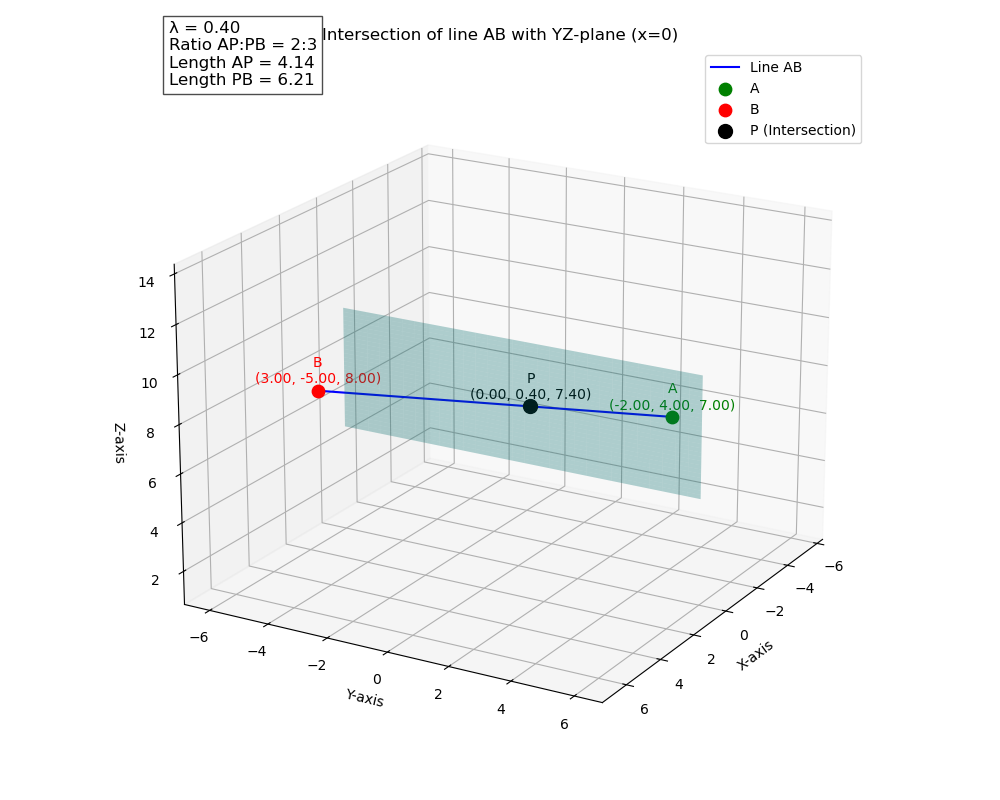
\includegraphics[width=0.9\columnwidth]{figs/Fig -62.png}
    \caption{}
    \label{fig:placeholder}
\end{figure}
\end{document}
